\subsection{Arquitectura}
A aplicação de Download está dividida em três partes: Download, Args e Connection.

\subsubsection{Args}
Neste módulo é feito o processamento dos argumentos da aplicação download. A partir da função parseArgs() é guardada a informação da URL dos argumentos do download para uma instância da struct args. No inicio da função são guardados os seguintes campos
\begin{itemize}
  \item Utilizador
  \item Palavra passe
  \item Host
  \item Path
\end{itemize}

No final são usadas as funções getIP() e getFileName() para, respetivamente, a partir do URL, usando a função gethostbyname(), saber o endereço IP do Host e o nome do Host, e para extrair, do último elemento do path, o nome do ficheiro que se vai descarregar, para no final do programa, ao criar o ficheiro transferido, saber que nome lhe atribuir.

\subsubsection{Connection}
Neste módulo temos como primeira função init(), que é encarregada de, ao receber um endereço IP e uma porta, criar um socket e iniciar a ligação a esse socket.

A função sendCommand() recebe um file descriptor de um socket e uma string com o comando a ser enviado. Com recurso á função send() de sockets, o comando é enviado para o servidor.

As funções readResponse() e readResponsePassive() usam getline() para esvaziar o buffer que contém a resposta do servidor. Em readResponse() há uma pequena verificação do código de resposta para, caso haja algum erro, o programa termine em vez de ficar bloqueado. Em readResponsePassive() é feito o processamento da resposta com o envio do commando pasv. A função retira da mensagem de resposta um endereço IP e uma porta que retorna a partir dos argumentos.

A função saveFile() está encarregue de criar o ficheiro que irá transferir para a máquina e preencher o ficheiro com os dados que recebe do servidor. Enquanto é feita a leitura dos dados, estes são adicionados ao ficheiro sequencialmente, até o buffer de leitura estar vazio.
\subsubsection{Download}
O módulo de download apenas contém a função main() com os passos necessários para fazer o download de um ficheiro.

O programa começa por verificar se apenas foi passado um argumento a partir da linha de comandos, caso isto não se verifique, é apresentada uma mensagem de erro e o programa termina. Se o programa receber um URL, este é passado por argumento para a função parseArgs() que preenche a struct args com os componentes do URL.

Uma lista de detalhes sobre a ligação é imprimida na consola e o programa continua a sua execução, chamando o predicado init(), que cria um socket para conseguir comunicar com o servidor. O programa procede com uma invocação de readResponse() para ler a mensagem de ligação e esvaziar o buffer de leitura.

Nesta altura inicia-se a sequência de login \cite{ftp_rfc}, na qual o programa envia o comando "user ." com um nome de utilizador, lê a resposta com readResponse() e executa as mesmas duas funções com o comando "pass .".
Caso não seja especificadas credenciais de login, o nome de utilizador usado é "anonymous" e a palavra passe usada é "1234". O programa executa o envio da palavra passe mesmo que não seja necessário, isto não afeta a troca de mensagens e simplifica o código.

o próximo comando a enviar é "pasv" para pedir ao servidor que transfira dados em modo passivo, o que faz com que seja necessário abrir outra ligação. A resposta a este comando é lida na função readResponsePassive() e contém o endereço IP e a porta á qual se realizará a nova ligação. Esta é feita via init() e devolve um novo file descriptor do socket de onde se retirará os dados.

Para finalizar é enviado o comando "retr [path]" com o caminho para o ficheiro e o programa chama a função saveFile() para guardar num ficheiro os dados lidos a partir do novo socket.

\begin{figure}[h]
    \centering
    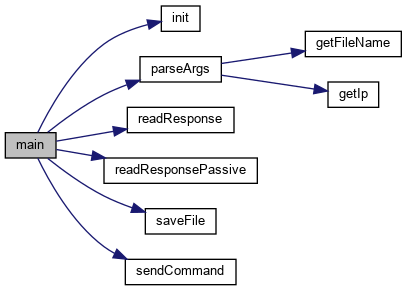
\includegraphics[width=0.5\textwidth]{imagens/function_call.png}
    \caption{Gráfico de chamadas de função para o download}
    \label{fig:callgraph}
\end{figure}